\documentclass[notitlepage,letterpaper,12pt]{article}% para articulo
% Este es un comentario <- Los comentarios comienzan con % 
% todo lo que se escriba hasta el final de la linea será ignorado <- Este es otro comentario

%Lenguaje del documento
\usepackage[english]{babel}% silabea palabras castellanas <- Puedo poner comentarios para explicar de que va este comando en la misma línea

%Encoding
\usepackage[utf8]{inputenc}% Acepta caracteres en castellano
\usepackage[T1]{fontenc}% Encoding de salida al pdf

%Triunfó el mal
\usepackage[normalem]{ulem}
\useunder{\uline}{\ul}{}
\providecommand{\e}[1]{\ensuremath{\times 10^{#1}}}

\usepackage{textcomp}
\usepackage{gensymb}


%Hipertexto
\usepackage[colorlinks=true,urlcolor=blue,linkcolor=blue]{hyperref}% navega por el doc: hipertexto y links

%Aquello de las urls
\usepackage{url} 

%simbolos matemáticos
\usepackage{amsmath}
\usepackage{amsfonts}
\usepackage{amssymb}
%\usepackage{physics} 

% permite insertar gráficos, imágenes y figuras, en pdf o en eps
\usepackage{graphicx}
\usepackage{epstopdf}
\usepackage{multirow}
\usepackage[export]{adjustbox}
% geometría del documento, encabezados y pies de páginas, márgenes
\usepackage{geometry}     
\geometry{letterpaper}       % ... o a4paper o a5paper o ... 
\usepackage{fancyhdr} % encabezados y pies de pg
\pagestyle{fancy}
\chead{\bfseries {}}
\lhead{} % si se omite coloca el nombre de la seccion
%\rhead{fecha del doc}
\lfoot{\it Métodos Computacionales: Tarea 5}
\cfoot{ }
\rfoot{Universidad de los Andes}
%\rfoot{\thepage}
%margenes
\voffset = -0.25in
\textheight = 8.0in
\textwidth = 6.5in
\oddsidemargin = 0.in
\headheight = 20pt
\headwidth = 6.5in
\renewcommand{\headrulewidth}{0.5pt}
\renewcommand{\footrulewidth}{0,5pt}

\begin{document}
\title{Métodos Computacionales: Tarea 5}
\author{
\textbf{Javier Alejandro Acevedo Barroso\thanks{e-mail: \texttt{ja.acevedo12@uniandes.edu.co}}}\\
\textit{Universidad de los Andes, Bogotá, Colombia}\\
} % Hasta aquí llega el bloque "author" (son dos autores por informe, orden alfabético)

%\date{Versión $\alpha \beta$ fecha del documento }
\maketitle %Genera el título del documento


\newpage
%Introducción
\section{Canal Iónico}

Mediante MCMC se calculó el circulo más grande posible en en plano con moléculas dadas a partir de un archivo de texto. Se graficó tanto el plano con las moléculas y el círculo más grande entre ellas, como el histograma en 2d del camino tomado por el MCMC.

\subsection{Primer archivo de datos}
La gráfica tiene la referencia \ref{g1d1}, en caso de que se haya separado del texto.

\begin{figure}[h]
  \centering
   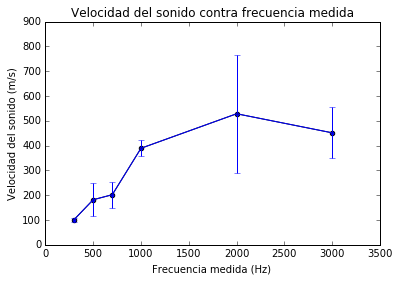
\includegraphics[scale= 0.5]{g1.png}
  \caption{Gráfica del plano de moléculas junto al poro propuesto (círculo más grande) entre ellas para el primer archivo de datos. Se puede observar que el círculo respeta el 1\AA  del radio de las moléculas. La gráfica incluye los resultados finales obtenido en el .c}
  \label{g1d1}
\end{figure}
\newpage

El histograma tiene referencia \ref{g2d1}
\begin{figure}[h]
  \centering
   \includegraphics[scale= 0.8]{his1.png}
  \caption{Histograma de las coordenadas $x$,$y$ para el centro del círculo. Es notorio que el histograma tiende rápidamente a la posición final del círculo. Si hubiera varias posibles posiciones o varias posiciones con radios no muy diferentes. Para el primer archivo de texto la caminata merodeó solo por una región. }
  \label{g2d1}
\end{figure}

\newpage

\subsection{Segundo archivo de datos}
La gráfica tiene referencia \ref{g1d2}

\begin{figure}[h]
  \centering
   \includegraphics[scale= 0.5]{g2.png}
  \caption{Gráfica del plano de moléculas junto al poro propuesto (círculo más grande) entre ellas para el segundo archivo de datos. Se puede observar que el círculo respeta el 1\AA  del radio de las moléculas. La gráfica incluye los resultados finales obtenido en el .c. La posición del centro del circulo depende fuertemente de la ejecución, pues hay dos regiones separadas con resultados muy similares}
  \label{g1d2}
\end{figure}
\newpage
El histograma tiene referencia \ref{his2}
\begin{figure}[h!]
  \centering
   \includegraphics[scale= 0.8]{his2.png}
  \caption{Histograma de las coordenadas $x$,$y$ para el centro del círculo. Es notorio que el histograma tiende rápidamente a la posición final del círculo. En el caso del segundo archivo de datos, la posición del círculo más grande depende de cada ejecución. Existen dos posiciones donde el radio máximo es bastante cercano, al mirar el histograma, se observa que la caminata merodea las dos posiciones. La posición del circulo de la gráfica anterior puede ser cualquiera de las dos pues son valores muy cercanos. }
  \label{his2}
\end{figure}

\newpage
\section{Carga de un Circuito RC}
A continuación las gráficas generadas en la determinación baynesiada de parámetros con MCMC.
Notando que no se hizo el walk directamente con $C$ y $R$ sino con $Q_{max}$ y $\tau$ tal que $Q_{max} = 10C$ y $\tau = \frac{1}{RC}$.

Las gráficas obtenidos fueron:
\begin{itemize}
\item Gráfica de los datos del circuito junto al modelo ajustado: \ref{reg}
\item Histograma del walk de R obtenido indirectamente a partir del walk de $\tau$ de del también obtenido indirectamente walk de $C$: \ref{histR}
\item Histograma del walk de $C$ obtenido indirectamente dividiendo $Q_{max}$ entre 10: \ref{hisC} 
\item Scatter del recorrido tomado por $Q_{max}$ y $\tau$. Este fue el recorrido realmente utilizado en el MCMC: \ref{QT}
\item Scatter del recorrido tomado por $R$ y $C$. Este recorrido se obtuvo indirectamente del recorrido anterior: \ref{QT}
\item Scatter de la verosimilitud del modelo con contra C: \ref{verC}
\item Scatter de la verosimilitud del modelo contra R: \ref{verR}
\end{itemize}



\begin{figure}[h!]
  \centering
   \includegraphics[scale= 0.8]{reg.png}
  \caption{Gráfica de los datos del circuito junto con el aj+uste utilizando determinación baynesiana de parámetros. Los parámetros obtenidoss se encuentra en la gráfica. }
  \label{reg}
\end{figure}

\begin{figure}[h!]
  \centering
   \includegraphics[scale= 0.8]{histR.png}
  \caption{Histograma del walk de R. Propiamente dicho, el walk de R fue indirecto pues se iteró sobre $Q_{max}$ y $\tau$ y se operó sobre cada elemento para obtener el walk de  R.}
  \label{histR}
\end{figure}

\begin{figure}[h!]
  \centering
   \includegraphics[scale= 0.8]{hisC.png}
  \caption{Histograma del walk de C. Propiamente dicho, el walk de C fue indirecto pues se iteró sobre $Q_{max}$ y $\tau$ y dividiendo $Q_{max}$ por 10 se obtuvo $C$. }
  \label{hisC}
\end{figure}

\begin{figure}[h!]
  \centering
   \includegraphics[scale= 0.8]{QT.png}
  \caption{Recorrido de $Q_{max}$ contra recorrido de $\tau$. Estos fueron los recorridos obtenidos directamente del MCMC. Los demás recorridos se obtuvieron a partir de estos.}
  \label{QT}
\end{figure}

\begin{figure}[h!]
  \centering
   \includegraphics[scale= 0.8]{RC.png}
  \caption{Recorrido de $R$ contra recorrido de $C$. Estos recorridos se obtuvieron indirectamente.}
  \label{RC}
\end{figure}

\begin{figure}[h!]
  \centering
   \includegraphics[scale= 0.8]{verC.png}
  \caption{Gráfica de la verosimilitud del modelo contra $C$. Las regiones con mayor verosimilitud es donde $C$ tiende a estar. Usualmente cerca a 9.}
  \label{verC}
\end{figure}

\begin{figure}[h!]
  \centering
   \includegraphics[scale= 0.8]{verR.png}
  \caption{Gráfica de la verosimilitud del modelo contra $R$. Las regiones con mayor verosimilitud es donde $R$ tiende a estar. Usualmente cerca a 5.}
  \label{verR}
\end{figure}






%\bibliographystyle{unsrt} % estilo de las referencias 
%\bibliography{mybib.bib} %archivo con los datos de los artículos citados


%\bibliography{mybib.bib} %archivo con los datos de los artículos citados

% Forma Manual de hacer las referencias
% Se escribe todo a mano...
% Descomentar y jugar

%\begin{thebibliography}{99}
%\bibitem{Narasimhan1993}Narasimhan, M.N.L., (1993), \textit{Principles of
%Continuum Mechanics}, (John Willey, New York) p. 510.

%\bibitem{Demianski1985}Demia\'{n}ski M., (1985), \textit{Relativistic
%Astrophysics,} in International Series in Natural Philosophy, Vol 110, Edited
%by \textit{D. Ter Haar}, (Pergamon Press, Oxford).
%\end{thebibliography}


%Fin del documento
\end{document}
